\documentclass[10pt,DIV16,a4paper,abstract=true,twoside=semi,openright]
{scrreprt}
\usepackage[T1]{fontenc}
\usepackage[USenglish]{babel}
\usepackage[numbers, sort&compress]{natbib}
\usepackage{isabelle,isabellesym}
\usepackage{booktabs}
\usepackage{paralist}
\usepackage{graphicx}
\usepackage{amssymb}
\usepackage{xspace}
\usepackage{xcolor}
\usepackage{listings}
\lstloadlanguages{HTML}
\usepackage[]{mathtools}
\usepackage[pdfpagelabels, pageanchor=false, plainpages=false]{hyperref}
\lstdefinestyle{html}{language=XML,
  basicstyle=\ttfamily,
  commentstyle=\itshape,
  keywordstyle=\color{blue},
  ndkeywordstyle=\color{blue},
}
\lstdefinestyle{displayhtml}{style=html,
  floatplacement={tbp},
  captionpos=b,
  framexleftmargin=0pt,
  basicstyle=\ttfamily\scriptsize,
  backgroundcolor=\color{black!2},
  frame=lines,
}
\lstnewenvironment{html}[1][]{\lstset{style=displayhtml, #1}}{}
\def\inlinehtml{\lstinline[style=html, columns=fullflexible]}

\pagestyle{headings}
\isabellestyle{default}
\setcounter{tocdepth}{1}
\newcommand{\ie}{i.\,e.\xspace}
\newcommand{\eg}{e.\,g.\xspace}
\newcommand{\thy}{\isabellecontext}
\renewcommand{\isamarkupsection}[1]{%
  \begingroup% 
  \def\isacharunderscore{\textunderscore}%
  \section{#1 (\thy)}%
  \endgroup% 
}

\title{Shadow DOM\\\medskip \Large 
  A Formal Model of the Document Object Model \emph{with Shadow Roots}}%



\author{%
  \href{https://www.brucker.ch/}{Achim~D.~Brucker}\footnotemark[1]
  \and
  \href{https://www.michael-herzberg.de/}{Michael Herzberg}\footnotemark[2]
}  

\publishers{
  \footnotemark[1]~Department of Computer Science, University of Exeter, Exeter, UK\texorpdfstring{\\}{, }
  \texttt{a.brucker@exeter.ac.uk}\\[2em]
  %
  \footnotemark[2]~  Department of Computer Science, The University of Sheffield, Sheffield, UK\texorpdfstring{\\}{, }
   \texttt{msherzberg1@sheffield.ac.uk}
}
\begin{document}
  \maketitle
  \begin{abstract}
    \begin{quote}
      In this AFP entry, we extend our formalization of the core DOM
      (AFP entry \href{https://www.isa-afp.org/entries/Core_DOM.html}
      {Core\_DOM}) with \emph{Shadow Roots}. Shadow roots are a recent
      proposal of the web community to support a component-based
      development approach for client-side web applications. 

      Shadow roots are a significant extension to the DOM standard
      and, as web standards are condemned to be backward compatible,
      such extensions often result in complex specification that may
      contain unwanted subtleties that can be detected by a
      formalization.

      Our Isabelle/HOL formalization is, in the sense of
      object-orientation, an extension of our formalization of the
      core DOM and enjoys the same basic properties, i.e., it is
      \begin{inparaenum}
        \item \emph{extensible}, i.e., can be extended without the need of
              re-proving already proven properties and
        \item \emph{executable}, i.e., we can generate executable code
          from our specification.
      \end{inparaenum}
      We exploit the executability to show that our formalization
      complies to the official standard of the W3C, respectively,
      the WHATWG.

      \bigskip
      \noindent{\textbf{Keywords:}} 
      Document Object Model, DOM, Shadow Root, Web Component, Formal
      Semantics, Isabelle/HOL
    \end{quote}
  \end{abstract}


\tableofcontents
\cleardoublepage

\chapter{Introduction}

In a world in which more and more applications are offered as services
on the internet, web browsers start to take on a similarly central
role in our daily IT infrastructure as operating systems. Thus, web
browsers should be developed as rigidly and formally as operating
systems. While formal methods are a well-established technique in the
development of operating systems (see,
\eg,~\citet{klein:operating:2009} for an overview of formal
verification of operating systems), there are few proposals for
improving the development of web browsers using formal
approaches~\cite{gardner.ea:dom:2008,raad.ea:dom:2016,jang.ea:establishing:2012,bohannon.ea:featherweight:2010}.

In~\cite{brucker.ea:afp-core-dom:2018}, we formalized the core of the
Document Object Model (DOM) in Isabelle/HOL\@. The
DOM~\cite{whatwg:dom:2017,w3c:dom:2015} is \emph{the} central data
structure of all modern web browsers. In this work, we extend the
formalization presented in~\cite{brucker.ea:afp-core-dom:2018} with
support for \emph{shadow trees}. Shadow trees are a recent addition to
the DOM standard~\cite{whatwg:dom:2017} that promise support for web
components. As we will see, this promise is not fully achieved and,
for example, the DOM standard itself does not formally define what a
component should be. In this work, we focus on a standard compliant
representation of the DOM with shadow
trees. As~\cite{brucker.ea:afp-core-dom:2018}, our formalization has
the following properties:
\begin{itemize}
\item It provides a \emph{consistency guarantee.} Since all
  definitions in our formal semantics are conservative and all rules
  are derived, the logical consistency of the DOM node-tree is reduced
  to the consistency of HOL.
\item It serves as a \emph{technical basis for a proof system.}  Based
  on the derived rules and specific setup of proof tactics over
  node-trees, our formalization provides a generic proof environment
  for the verification of programs manipulating node-trees.
\item It is \emph{executable}, which allows to validate its compliance
  to the standard by evaluating the compliance test suite on the
  formal model and
\item It is \emph{extensible} in the sense
  of~\cite{brucker.ea:extensible:2008-b,brucker:interactive:2007},
  \ie, properties proven over the core DOM do not need to be re-proven
  for object-oriented extensions such as the HTML document model.
\end{itemize}

In this AFP entry, we limit ourselves to the faithful formalization of
the DOM. As the DOM standard does not formally define web components,
we address the question of formally defining web components and
discussing their safety properties
elsewhere~\cite{brucker.ea:afp-dom-components:2020,brucker.ea:web-components:2019}.

The rest of this document is automatically generated from the
formalization in Isabelle/HOL, i.e., all content is checked by
Isabelle (we refer readers interested in a more high-level presentation 
and additional explanations to~\cite{herzberg:web-components:2020,brucker.ea:web-components:2019}. 
The structure follows the theory dependencies 
(see \autoref{fig:session-graph}): first, we
formalize the DOM with Shadow Roots (\autoref{cha:dom}) and then
formalize we the relevant compliance test cases in
\autoref{cha:tests}.

\begin{figure}
  \centering
  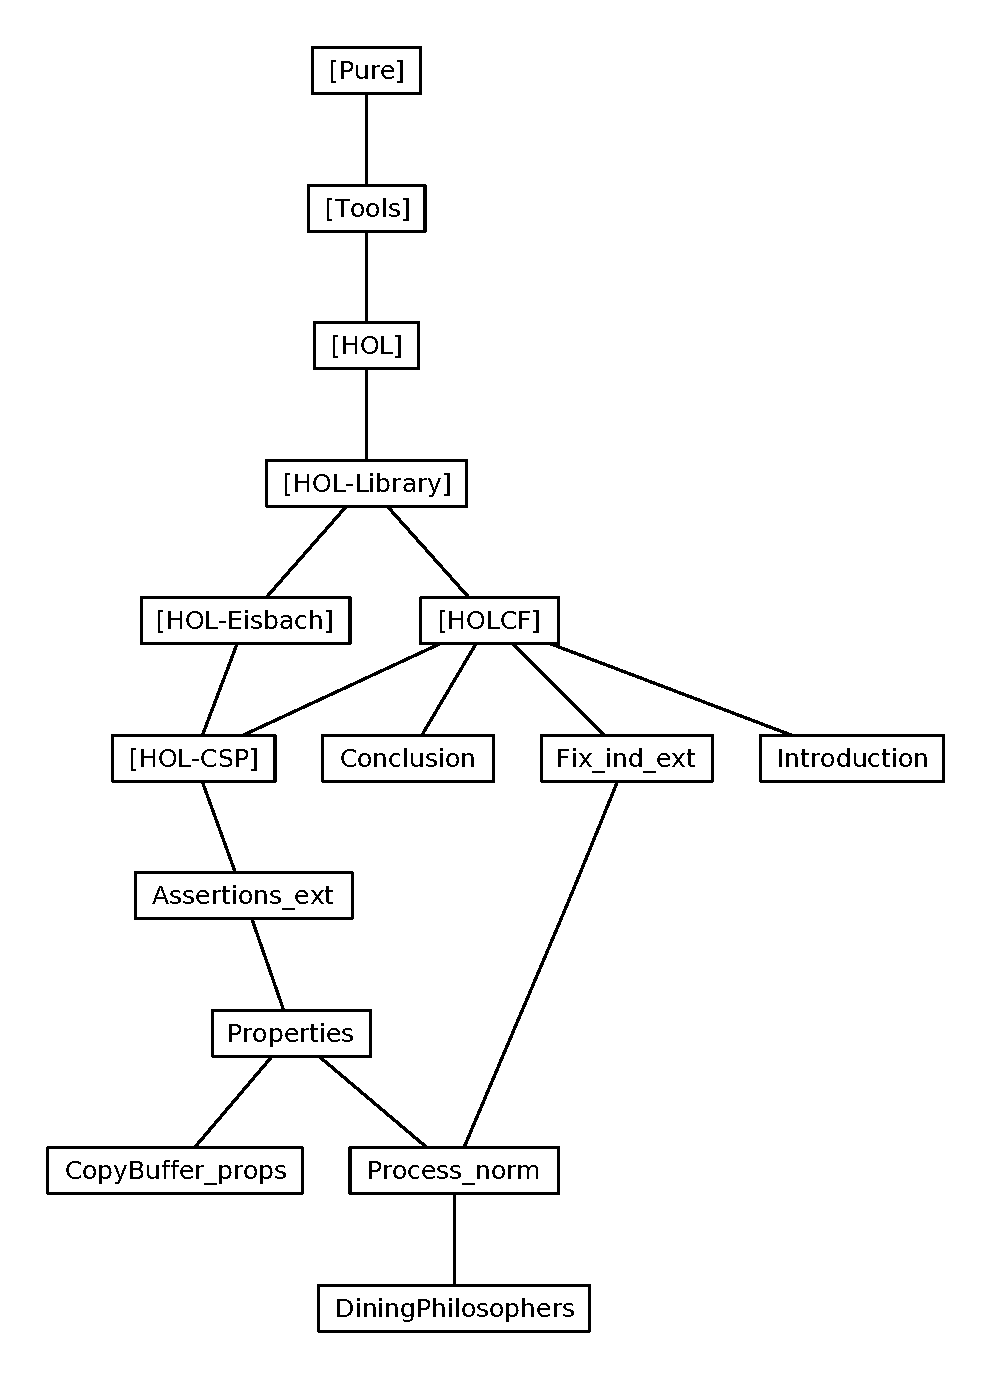
\includegraphics[height=.9\textheight]{session_graph}
  \caption{The Dependency Graph of the Isabelle Theories.\label{fig:session-graph}}
\end{figure}

\clearpage

\chapter{The Shadow DOM}
\label{cha:dom}
In this chapter, we introduce the formalization of the core DOM
\emph{with Shadow Roots}, i.e., the most important algorithms for
querying or modifying the Shadow DOM, as defined in the standard.

\input{ShadowRootClass.tex}
\input{ShadowRootMonad.tex}
\input{Shadow_DOM.tex}


\chapter{Test Suite}
\label{cha:tests}
In this chapter, we present the formalized compliance test cases for
the core DOM. As our formalization is executable, we can
(symbolically) execute the test cases on top of our model. Executing
these test cases successfully shows that our model is compliant to the
official DOM standard. As future work, we plan to generate test cases
from our formal model (e.g.,
using~\cite{brucker.ea:interactive:2005,brucker.ea:theorem-prover:2012})
to improve the quality of the official compliance test suite. For more
details on the relation of test and proof in the context of web
standards, we refer the reader to
\cite{brucker.ea:standard-compliance-testing:2018}.

\input{Shadow_DOM_BaseTest.tex}
\input{slots.tex}
\input{slots_fallback.tex}
\input{Shadow_DOM_Document_adoptNode.tex}
\input{Shadow_DOM_Document_getElementById.tex}
\input{Shadow_DOM_Node_insertBefore.tex}
\input{Shadow_DOM_Node_removeChild.tex}
\input{Shadow_DOM_Tests.tex}


{\small
  \bibliographystyle{abbrvnat}
  \bibliography{root}
}
\end{document}

%%% Local Variables:
%%% mode: latex
%%% TeX-master: t
%%% End:
